\chapter{Angewandtes Beispiel}
{
Die Kosten Berechnung setzt sich aus \(F=G+H\) \\ G ist dabei Kosten vom Start und H sind die Kosten zum Ziel. \\
Hier ist ein Beispiel das das Pathfinding von einem Auto zum Ziel Behandelt.
\begin{itemize}
    \item \color{violet} Gesperrte Zelle (Closed List)\color{black}
    \item \color{blue} Hinderniss\color{black}
    \item \color{green} Offene Zelle (Open List)
\end{itemize} 
}
\section{Ablauf}
{
\begin{minipage}{0.4\linewidth}
  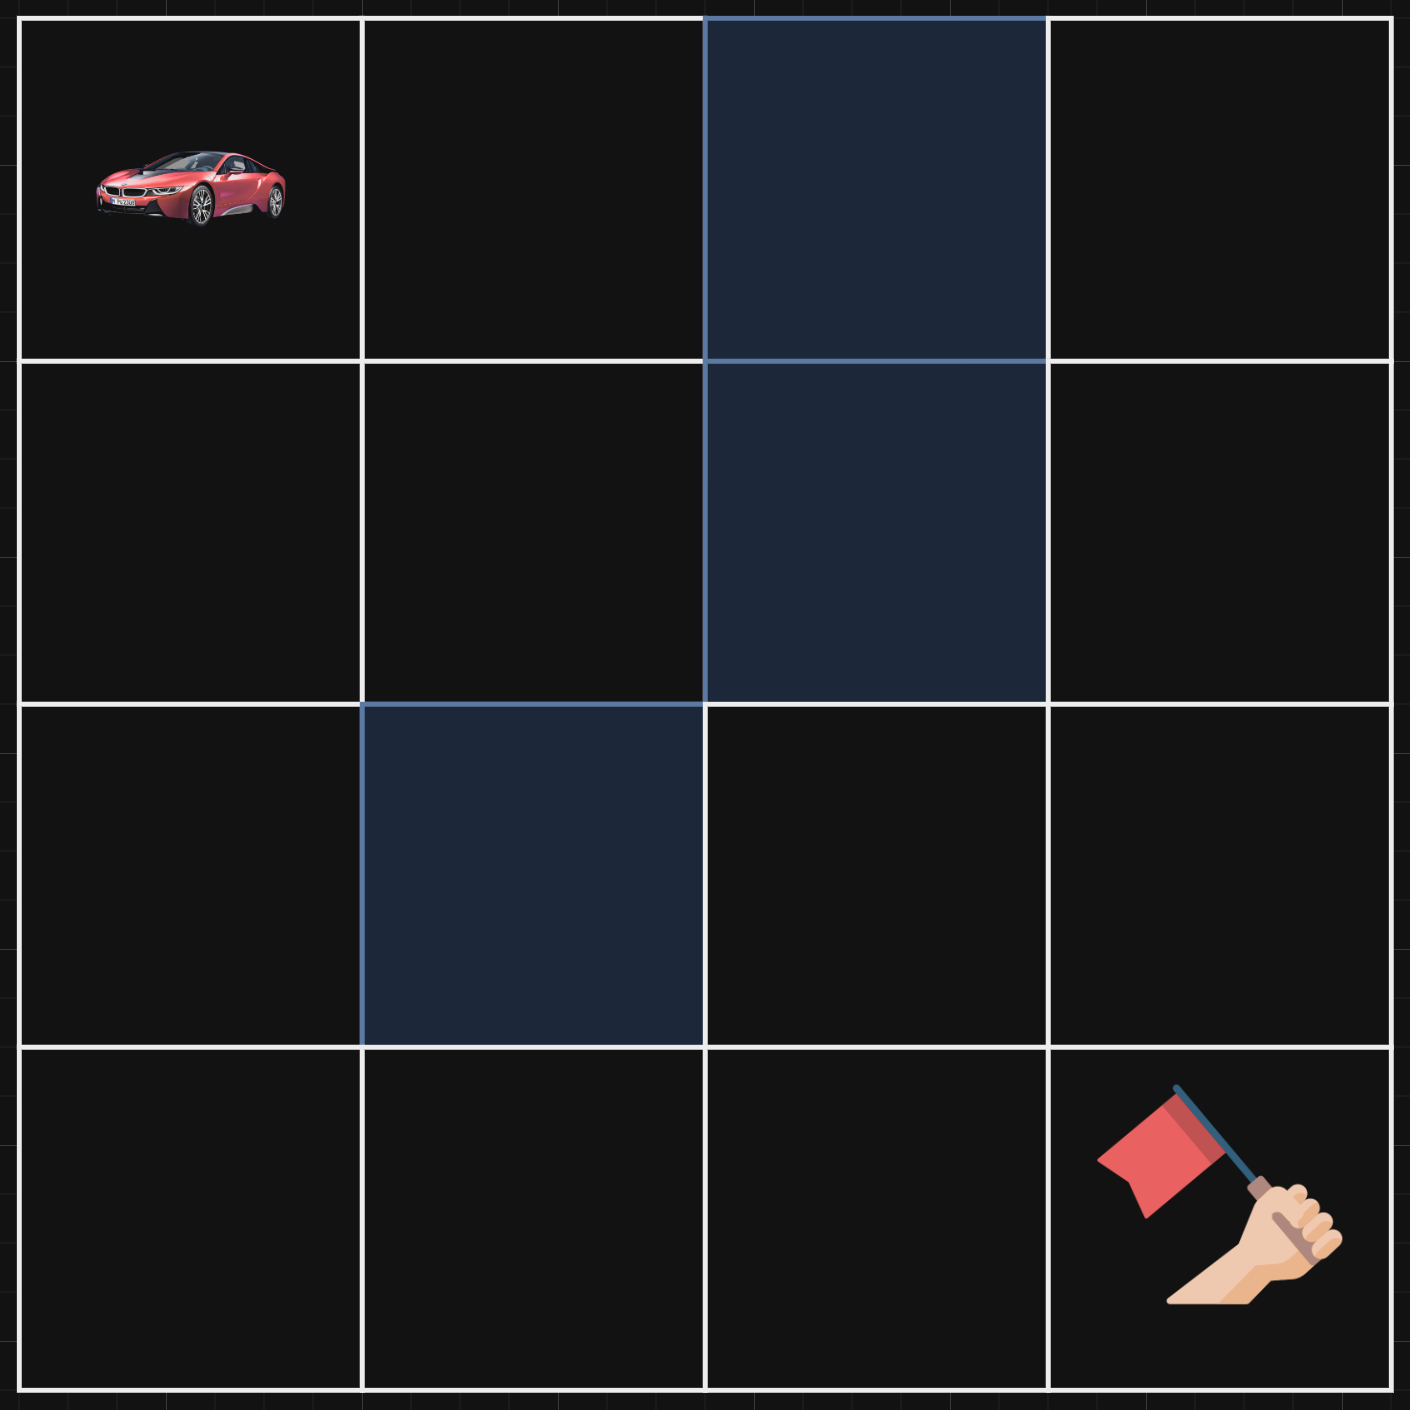
\includegraphics[scale=.125]{Cars/img1.png}
\end{minipage}
\begin{minipage}{0.6\linewidth}
Die Karte wird mit einem Start, einem Ziel und Hindernissen initialisiert
\end{minipage}
}
{
\begin{minipage}{0.4\linewidth}
  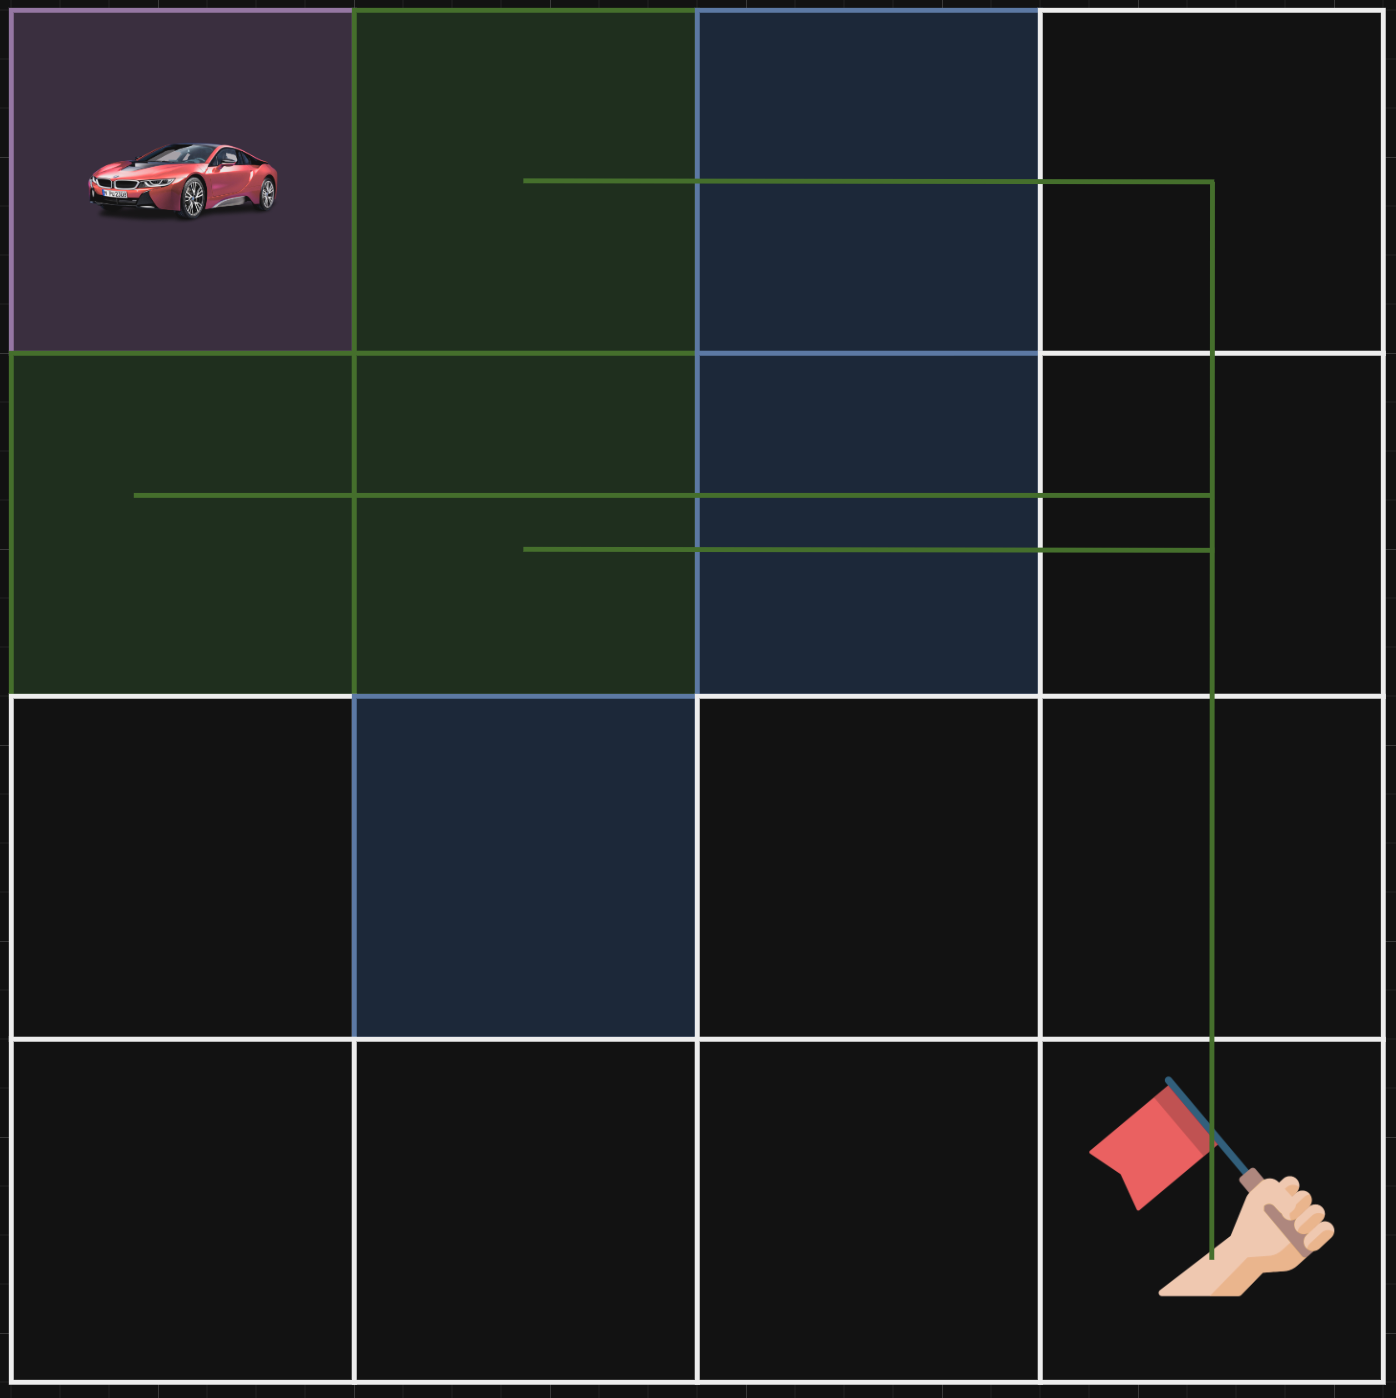
\includegraphics[scale=.125]{Cars/img2.png}
\end{minipage}
\begin{minipage}{0.6\linewidth}
Bei jedem Durchlauf wird das aktuelle Feld zur gesperrten Liste hinzugefügt.\\
Dann wird die ausgewählte Heuristik ausgewählt und damit der Weg von Start bis Ziel geschätzt grüne Linien.
Dann werden die Feld Kosten berechnet mit der Formel \(F=G+H\). Das Diagonal unten ist das Günstigste deswegen ist dies der nächste Schritt.
\end{minipage}
}
{
\begin{minipage}{0.4\linewidth}
  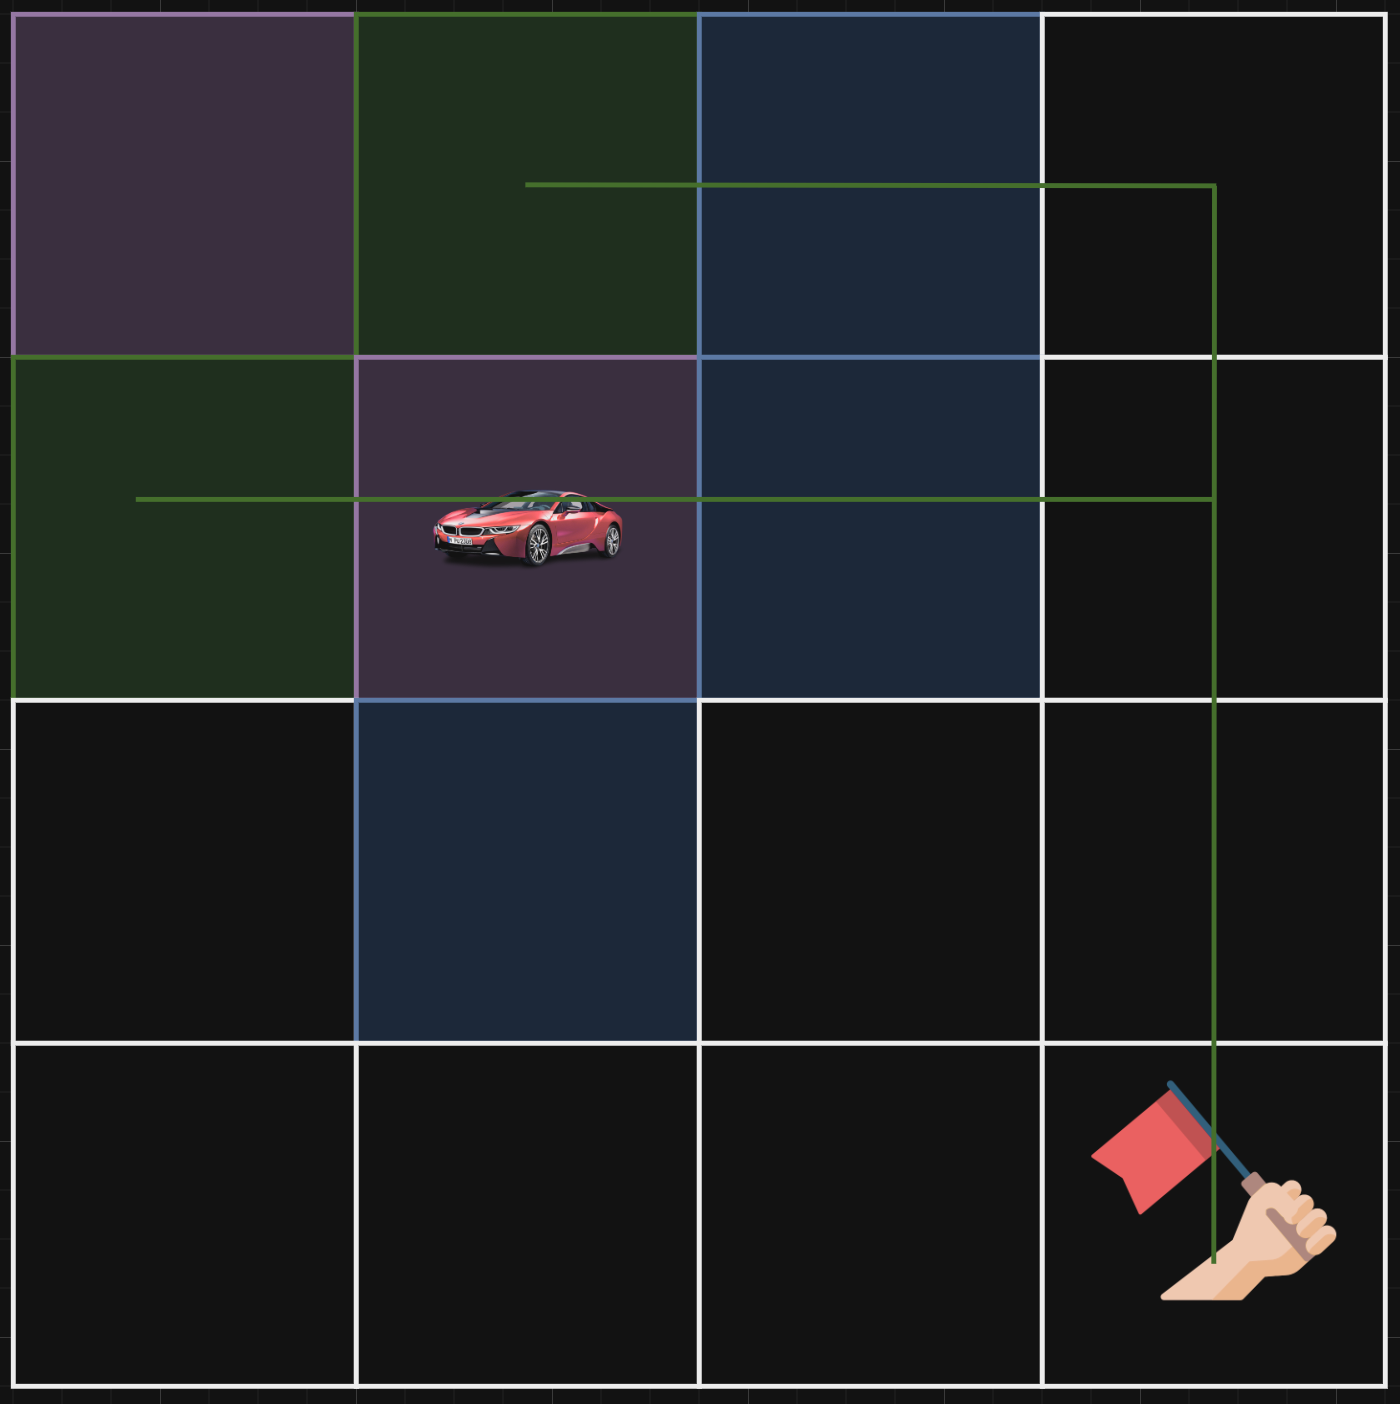
\includegraphics[scale=.125]{Cars/img3.png}
\end{minipage}
\begin{minipage}{0.6\linewidth}
Das aktuelle Feld wird wieder Gesperrt da die anderen beiden Felder schon zur Open List hinzugefügt wurden müssen nicht nochmal die Kosten berechnet werden. 
\end{minipage}
}
{
\begin{minipage}{0.4\linewidth}
  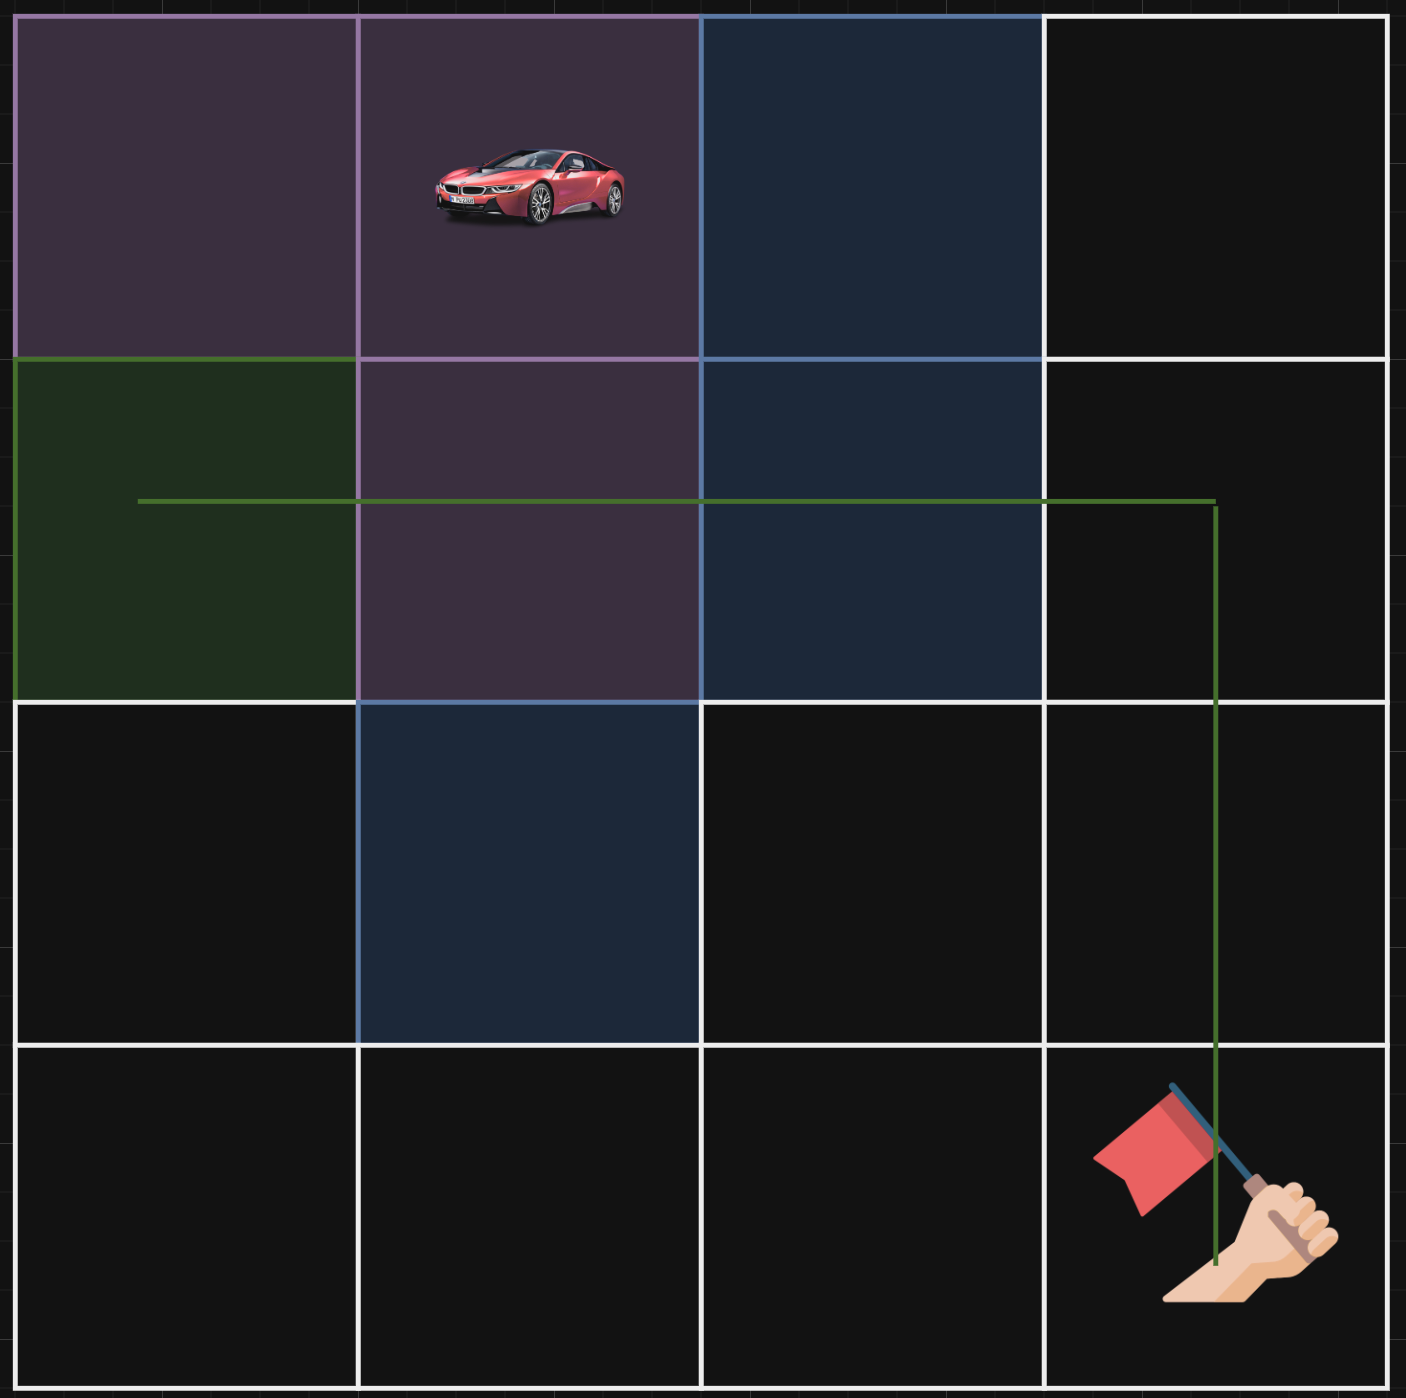
\includegraphics[scale=.125]{Cars/img4.png}
\end{minipage}
\begin{minipage}{0.6\linewidth}
Wenn eine Deadlock Sitatuation entsteht wird zu der nächsten Top Priority in der Open List gegangen und von dort aus weiter gesucht.
\end{minipage}
}
{
\begin{minipage}{0.4\linewidth}
  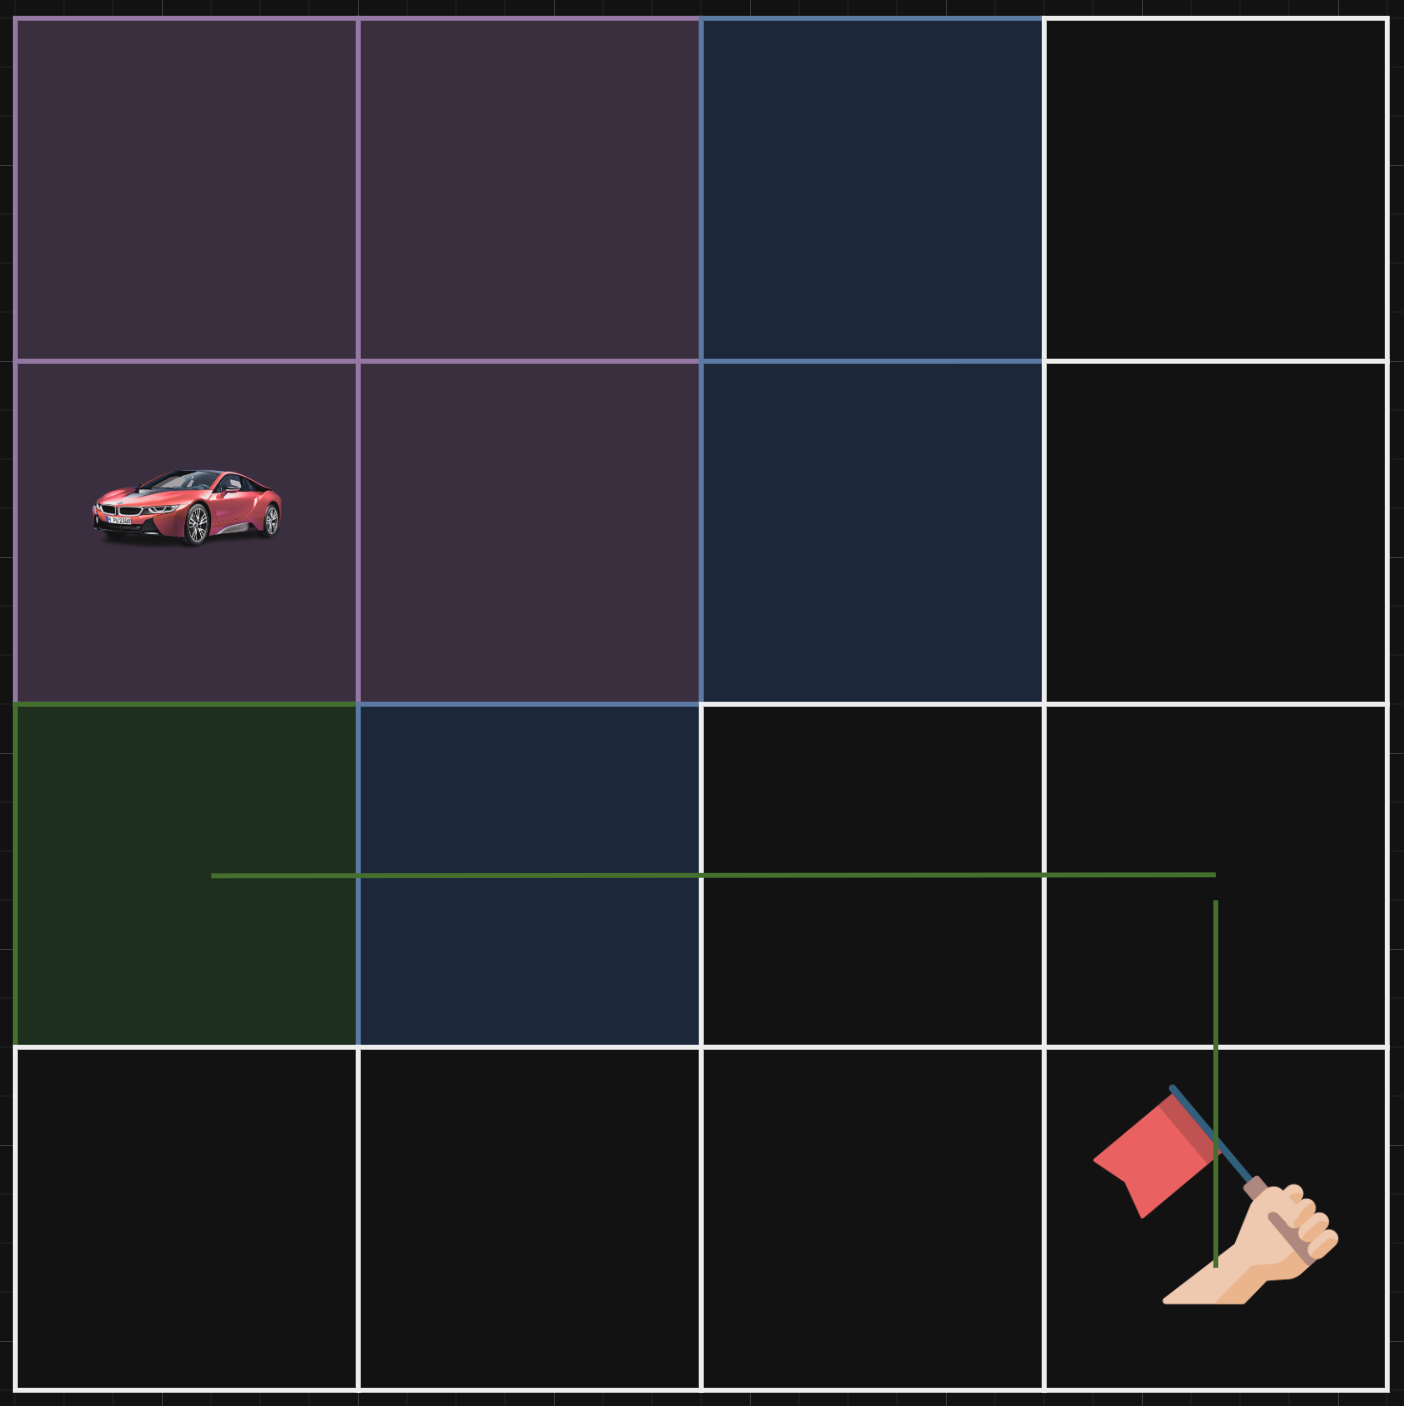
\includegraphics[scale=.125]{Cars/img5.png}
\end{minipage}
\begin{minipage}{0.6\linewidth}
Das Feld wird wieder zur Closed List hinzugefügt. Das Einzige Mögliche Feld wird zur Open List hinzugefügt. Bei de Manhattan Heuristik hätte das Feld den Wert \(H=40\) und \(G=20\). Also insgesamt Kosten von 60.
\end{minipage}
}
{
\begin{minipage}{0.4\linewidth}
  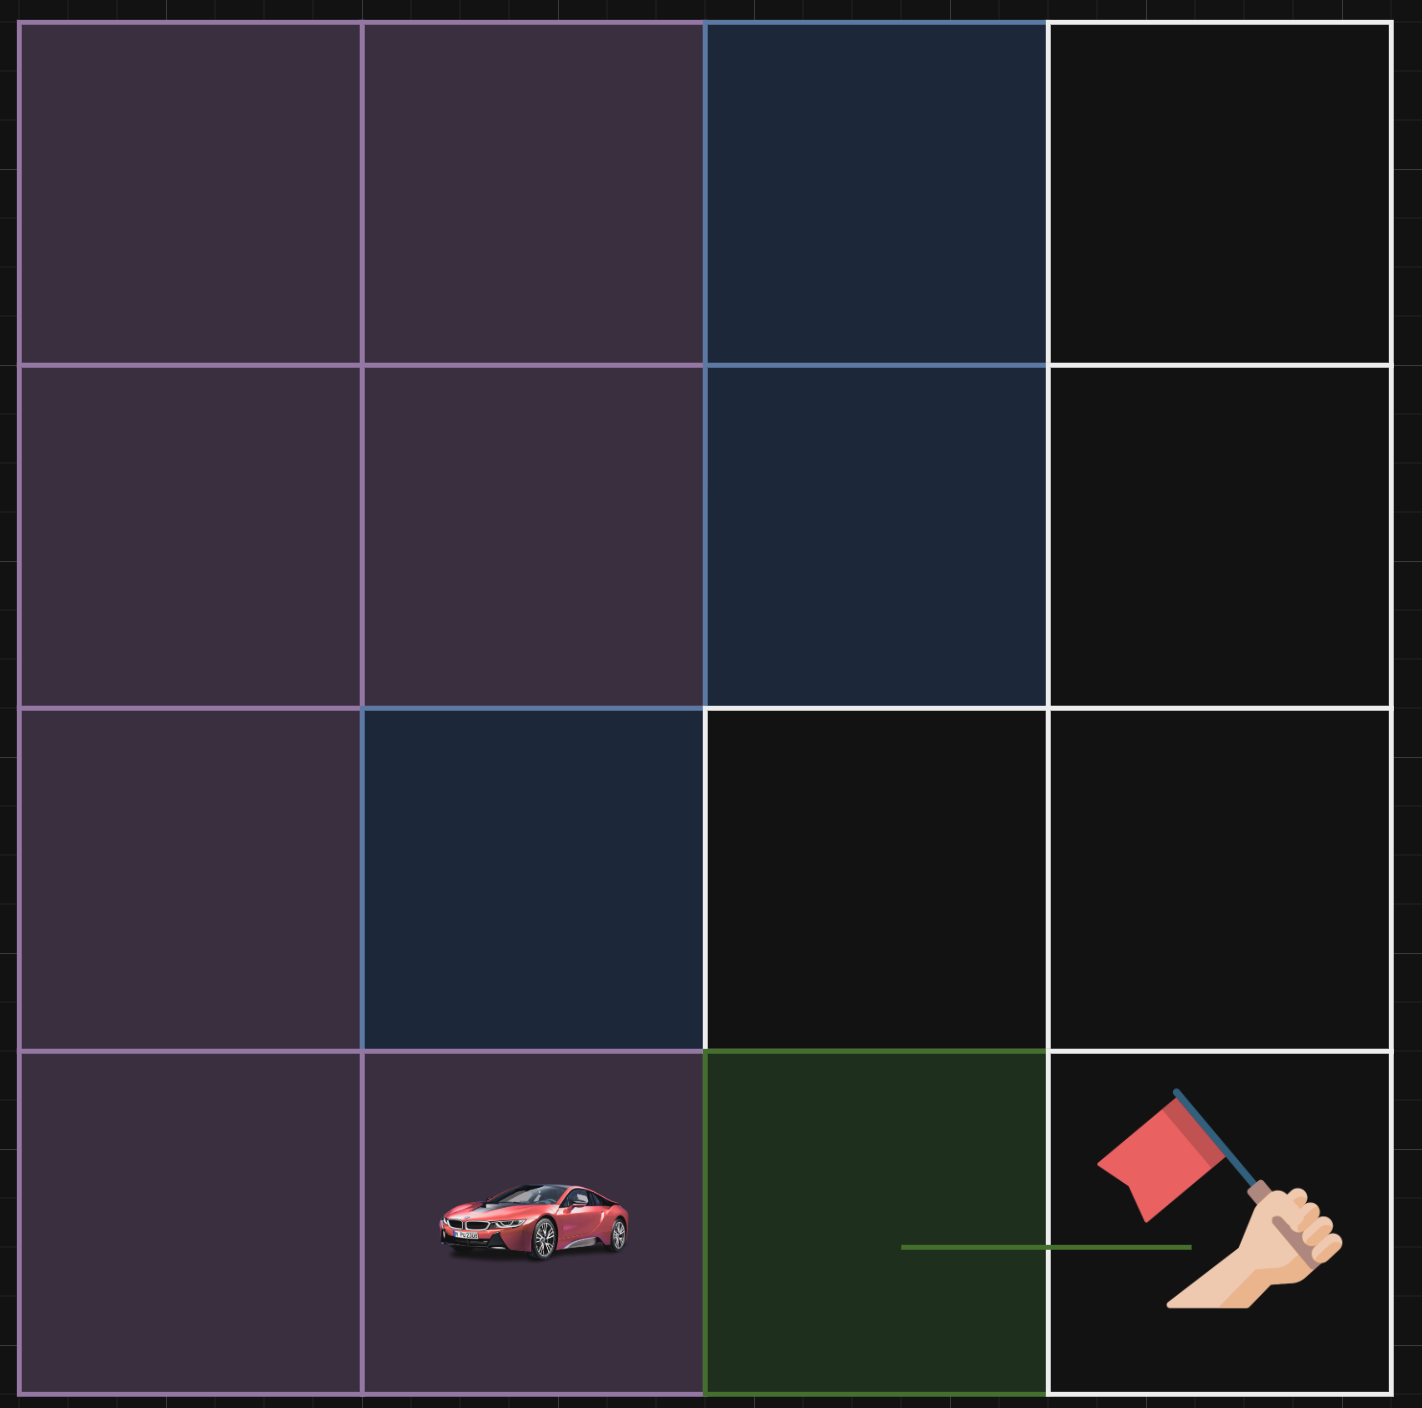
\includegraphics[scale=.125]{Cars/img6.png}
\end{minipage}
\begin{minipage}{0.6\linewidth}
Es kann nur diagonal gegangen werden wenn die \(x\) und die \(y\) Richtung frei sind. 

Diagonal gehen kostet 14 da die Quadratwurzel aus
\(\sqrt{2}=1.41...\) 
\end{minipage}
}
{
\begin{minipage}{0.4\linewidth}
  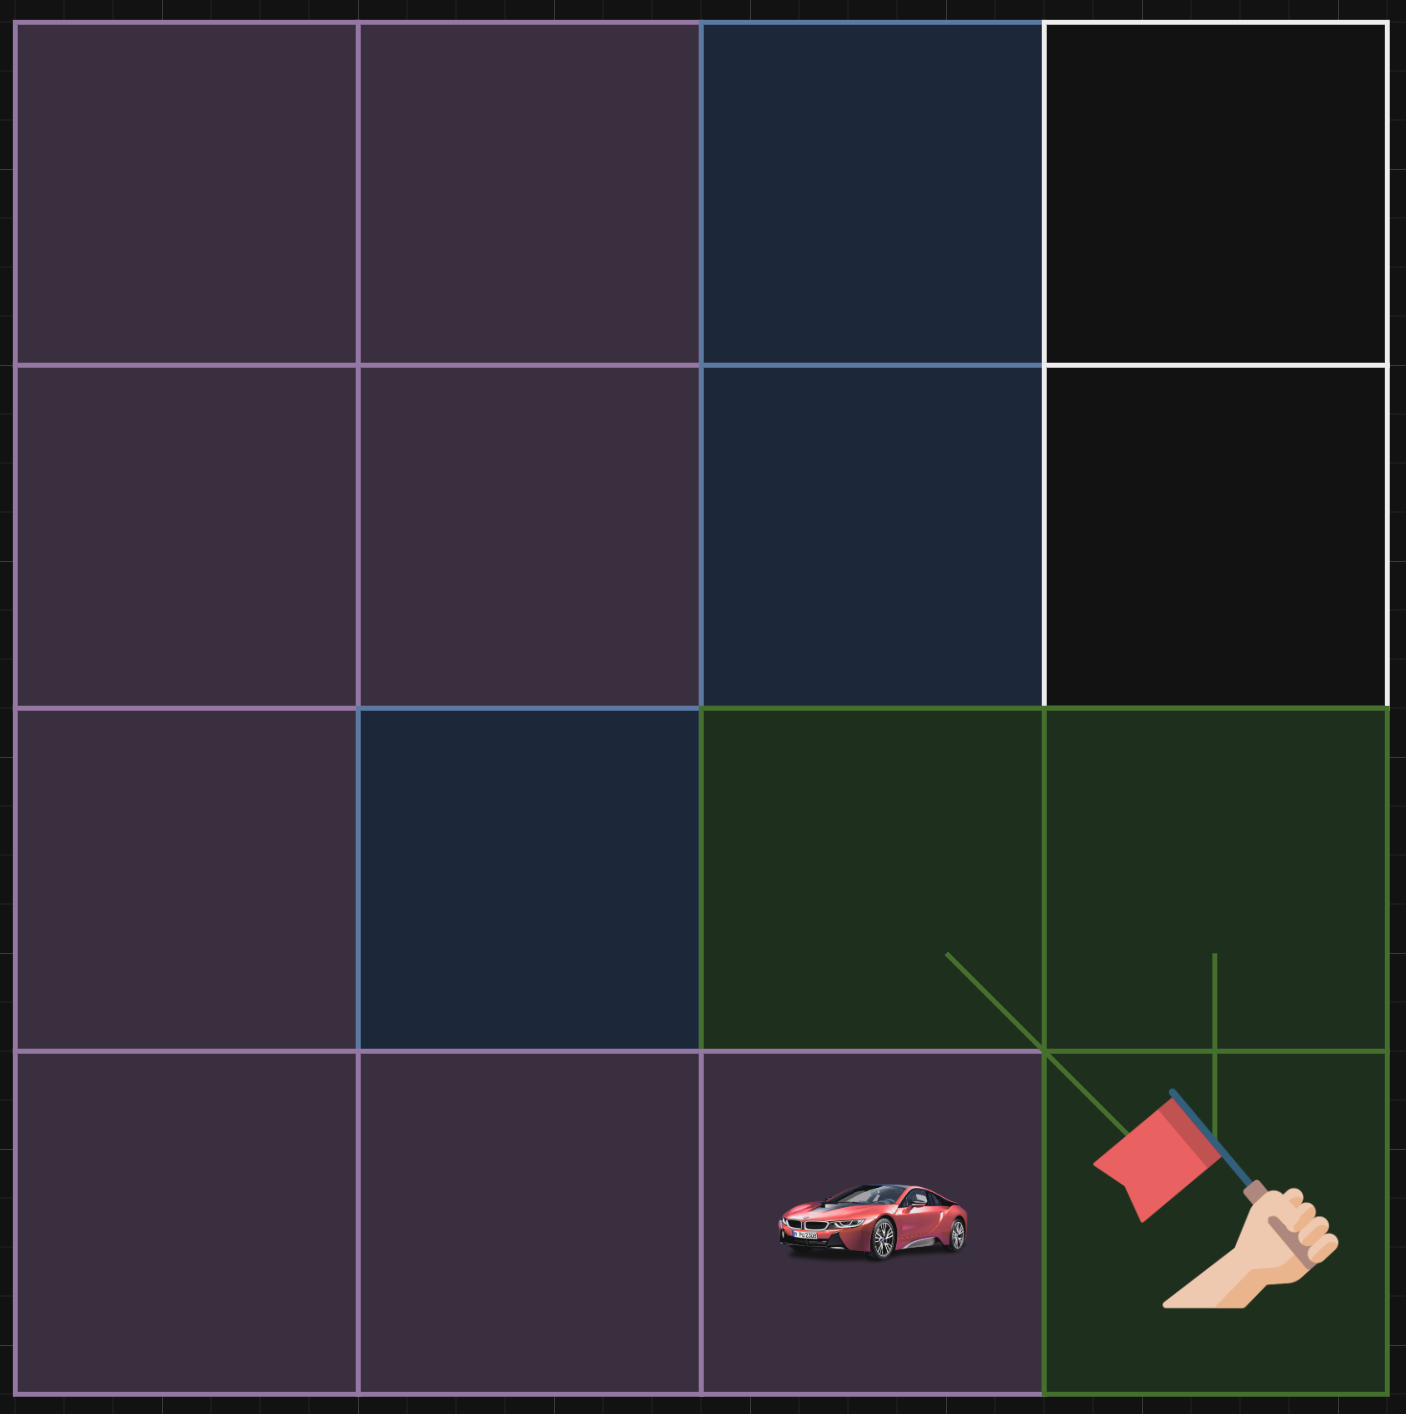
\includegraphics[scale=.125]{Cars/img7.png}
\end{minipage}
\begin{minipage}{0.6\linewidth}
Wenn das Ziel in der Open List steht ist es erreicht.
\end{minipage}
}
{
\begin{minipage}{0.4\linewidth}
  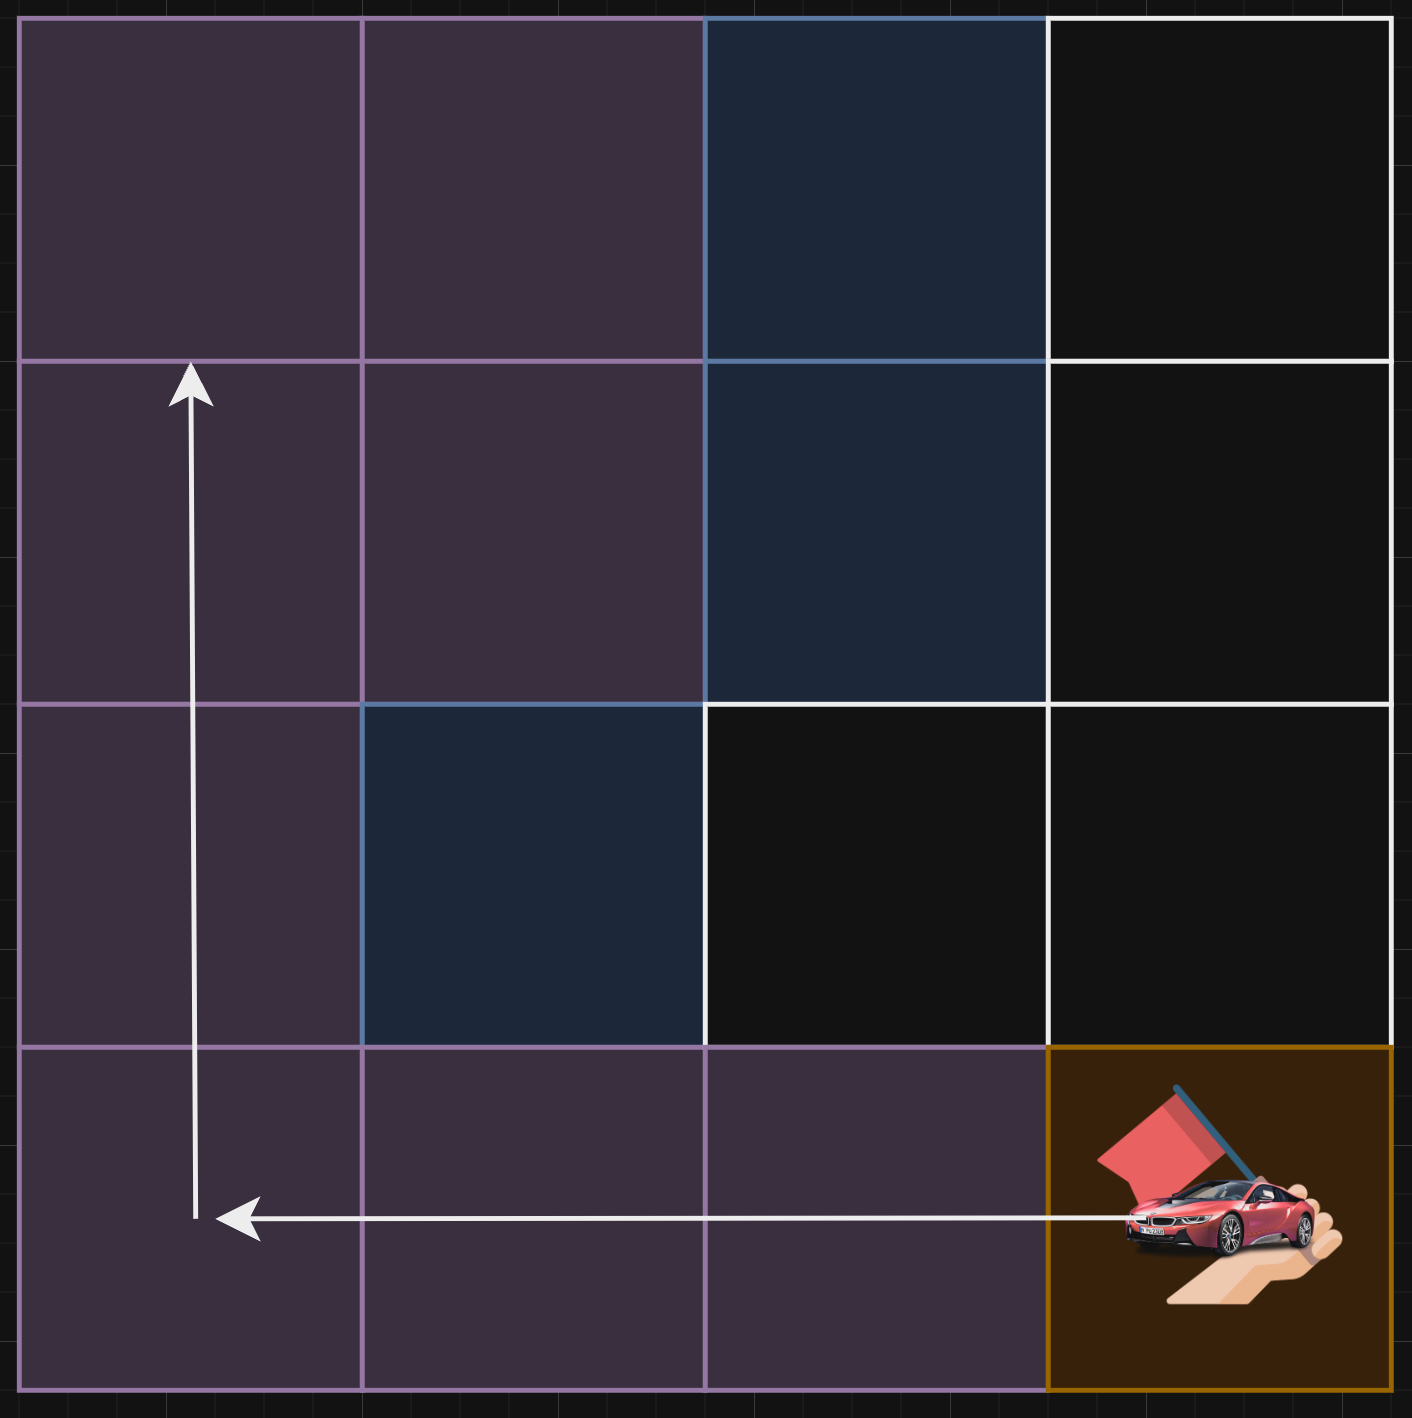
\includegraphics[scale=.125]{Cars/img8.png}
\end{minipage}
\begin{minipage}{0.6\linewidth}
Vom Ziel wird nun rückwärts der Kürzeste Pfad ausgewertet indem man den Parent der Felder nimmt die vom Start zum Ziel führen. Also man fängt man mit dem letzten Feld an und schaut wer dieses untersucht hat usw. Bis man am Start angekommen ist.
\end{minipage}
}




